\chapter{Regularization}
Le tecniche di regolarizzazione puntano a ridurre l'errore della loss function sul validation set e sul test set.

La regolarizzazione può avvenire:
\begin{itemize}
  \item Direttamente: cambiando i vincoli o la funzione obiettivo
  \item Indirettamente: aggiungendo dati
\end{itemize}

Un regolarizzatore efficace riduce significativamente la varianza mentre non aumenta molto il bias. 

\begin{figure}[ht]
  \centering
  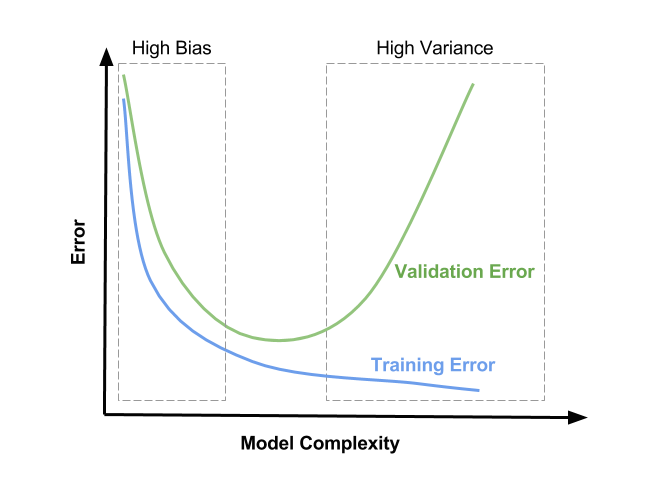
\includegraphics[width=0.8\linewidth]{images/Bias-Variance-Tradeoff-In-Machine-Learning-1.png}
  \caption{Bias-variance tradeoff example \cite{img:model-complexity}. High bias $\rightarrow$ underfitting,  High variance $\rightarrow$ overfitting}
\end{figure}

Controllare la complessità del modello non è semplice, non basta trovare la dimensione giusta il numero giusto di parametri.
Nel deep learning si basa su trovare il miglior modello che è un modello grande che è stato propriamente regolarizzato.

\section{Norm Penalities}
Si limita la capacità del modello aggiungendo una penalità $\Omega(\theta)$ alla funzione obiettivo $J$. 
%
\begin{align*}
  \tilde{J}(\theta) = J(\theta) + \alpha \Omega(\theta)
\end{align*}
%
$\alpha \in [0, \inf)$ è un iperparametro che pesa il contributo della \textbf{norm penalty} nella funzione obiettivo.

Solitamente la penalty $\Omega$ penalizza solo i pesi della trasformazione affine di ogni layer. 
I bias nella trasformazione affine richiedono meno dati per fittare, quindi non vengono regolarizzati.

Più parametri ci sono nel modello più questi sono sensibili a varianza, e quindi creano più instabilità nel modello.

- somma assoluta dei pesi
\begin{align*}
  \Omega(w, b) = \sum_{w_j}|w_j|
\end{align*}

- somma quadratica dei pesi
\begin{align*}
  \Omega(w, b) = \sqrt{\sum_{w_j}|w_j|^2}
\end{align*}

Data la funzione obiettivo seguente
\begin{align*}
  \tilde{J}(w; X, y) = \frac{\alpha}{2} w^T w + J(w; X, y)
\end{align*}

Il gradiente é:
\begin{align*}
  \nabla_w \tilde{J}(w; X, y) = \alpha w + \nabla_w J(w; X, y)
\end{align*}

La regola di aggiornamento dei pesi usando la norma L2 diventa la seguente
\begin{align*}
  w &= w - \epsilon \big( \alpha w + \nabla_w J(w; X, y) \big)\\
    &= (1 - \epsilon \alpha) w + \epsilon \nabla_w J(w; X, y)
\end{align*}
